                %%%%%%%%%%%%%%%%%%%%%%%%%%%%%%%%%%%%%%%%%%%%%%%%%%%%%%%%%%%%%%%%%%%%%
% LaTeX Template: Project Titlepage Modified (v 0.1) by rcx
%
% Original Source: http://www.howtotex.com
% Date: February 2014
% 
% This is a title page template which be used for articles & reports.
% 
% This is the modified version of the original Latex template from
% aforementioned website.
% 
%%%%%%%%%%%%%%%%%%%%%%%%%%%%%%%%%%%%%%%%%%%%%%%%%%%%%%%%%%%%%%%%%%%%%%

\documentclass[12pt]{report}
\usepackage[a4paper]{geometry}
\usepackage[myheadings]{fullpage}
\usepackage{fancyhdr}
\usepackage{lastpage}
\usepackage{graphicx, wrapfig, subcaption, setspace, booktabs}
\usepackage[T1]{fontenc}
\usepackage[font=small, labelfont=bf]{caption}
\usepackage{fourier}
\usepackage[protrusion=true, expansion=true]{microtype}
\usepackage[english]{babel}
\usepackage{sectsty}
\usepackage{verbatim}
\usepackage{url, lipsum}
\usepackage{amsmath}
\usepackage{graphicx}
\usepackage{listings}
\usepackage{enumitem}
\usepackage{float}
\usepackage{array}
\usepackage{adjustbox}
\usepackage{multirow}
\newcolumntype{L}{>{\centering\arraybackslash}m{3cm}}
\usepackage{titlesec}
\usepackage{hyperref}

\titleformat{\subsubsection}[runin]
  {\normalfont\normalsize\bfseries}{\thesection}{1em}{}
\newcommand{\HRule}[1]{\rule{\linewidth}{#1}}
\onehalfspacing
\setcounter{tocdepth}{5}
\setcounter{secnumdepth}{5}
\graphicspath{ {images/} }
\setlength\parindent{0pt}

%-------------------------------------------------------------------------------
% HEADER & FOOTER
%-------------------------------------------------------------------------------
\pagestyle{fancy}
\fancyhf{}
\setlength\headheight{15pt}
\fancyhead[L]{Homework 4}
\fancyhead[R]{CS 5785: Applied Machine Learning}
\fancyfoot[R]{Page \thepage\ of \pageref{LastPage}}
%-------------------------------------------------------------------------------
% TITLE PAGE
%-------------------------------------------------------------------------------

\begin{document}


\title{ \normalsize \textsc{CS 5785: Applied Machine Learning}
        \\ [2.0cm]
        \HRule{0.5pt} \\
        \LARGE \textbf{\uppercase{Final Exam Report}}
        \HRule{2pt} \\ [0.5cm]
        \normalsize \today \vspace*{5\baselineskip}}

\date{}

\author{
	Anonymous \\  \\  
        Cornell Tech }

\maketitle
\tableofcontents
\newpage

%-------------------------------------------------------------------------------
% Section title formatting
\sectionfont{\scshape}
%-------------------------------------------------------------------------------

%-------------------------------------------------------------------------------
% BODY
%-------------------------------------------------------------------------------

\section*{Description To Image Matching}
\addcontentsline{toc}{section}{Description To Image Matching}

\section*{Abstract}
\addcontentsline{toc}{section}{Abstract}
Matching search text to image results is a common use case of Machine Learning in image search. We constructed various statistical models to create mappings of text descriptions to images. For a given search query, these models output images sorted by some measure of the level of predicted similarity to the text. We explored various representations of the text data, different solution frameworks and experimental design to train our algorithm to accurately output image queries. \\

\section*{Introduction}
\addcontentsline{toc}{section}{Introduction}
Image retrieval involves indexing, storing and retrieving digital images using input search text or image. Typical approaches involve using ?context? around the images, such as tags, keywords or descriptions to retrieve images. There are also content-based image retrieval (CBIR) systems that use computer vision to extract information from images for use in image search. Clustering and image prototyping using image collection exploration and automatic summarization are other notable methods.

\subsection*{The Challenge}
\addcontentsline{toc}{subsection}{The Challenge}
Our task was to predict relevant images given a natural language search query. We were provided with a training set of 10,000 images along with corresponding lists of tags indicating objects in the image, feature vectors extracted using ResNet, an advanced convolutional neural network, and five-sentence descriptions. For evaluation, we were given a separate set of 2,000 images and matching tags and 2,000 five-sentence descriptions. For each image, we had to predict 20 relevant images, rank-ordered by relevance. Mean Average Precision at 20 (MAP@20) was used to evaluate the results based on the positioning of the actual image match within the output. 

\subsection*{Our Algorithm}
\addcontentsline{toc}{subsection}{Our Algorithm}



\section*{Experiment}
\addcontentsline{toc}{section}{Experiment}


\subsection*{Data Encoding}
\addcontentsline{toc}{subsection}{Data Encoding}

We explored various ways to represent the text description data for use in statistical techniques, such as Bag of Words and Document Vectors. \\

The bag of words approach is a common feature generation tool that involves representing text data as a bag of words that constitute it. Note that bag of words is an orderless representation of the text data. How words appear in relation to one another is not modeled in this representation. \\

In contrast, word vectors are numerical representations of relationships between words (e.g. man: woman $\rightarrow$ king: queen). Document vectors are an extension of the concept of word vectors, and represent documents in a corpus of text as vectors in an n-dimensional space. They are created using a shallow neural network that transforms cleaned and vectorized text data into a representative numerical feature vector, also called the embedding.\\

We ultimately chose to use Bag of Words for data encoding as this produced more accurate results in description matching. 



\subsection*{Approaches}
\addcontentsline{toc}{subsection}{Approaches}
Since we had to create mappings between test descriptions and test images, we explored multiple approaches to tackling this problem. \textbf{Figure 1} shows a mapping the data provided, which intuitively pointed us in a few directions. 


\begin{figure}[H]
   \centering
   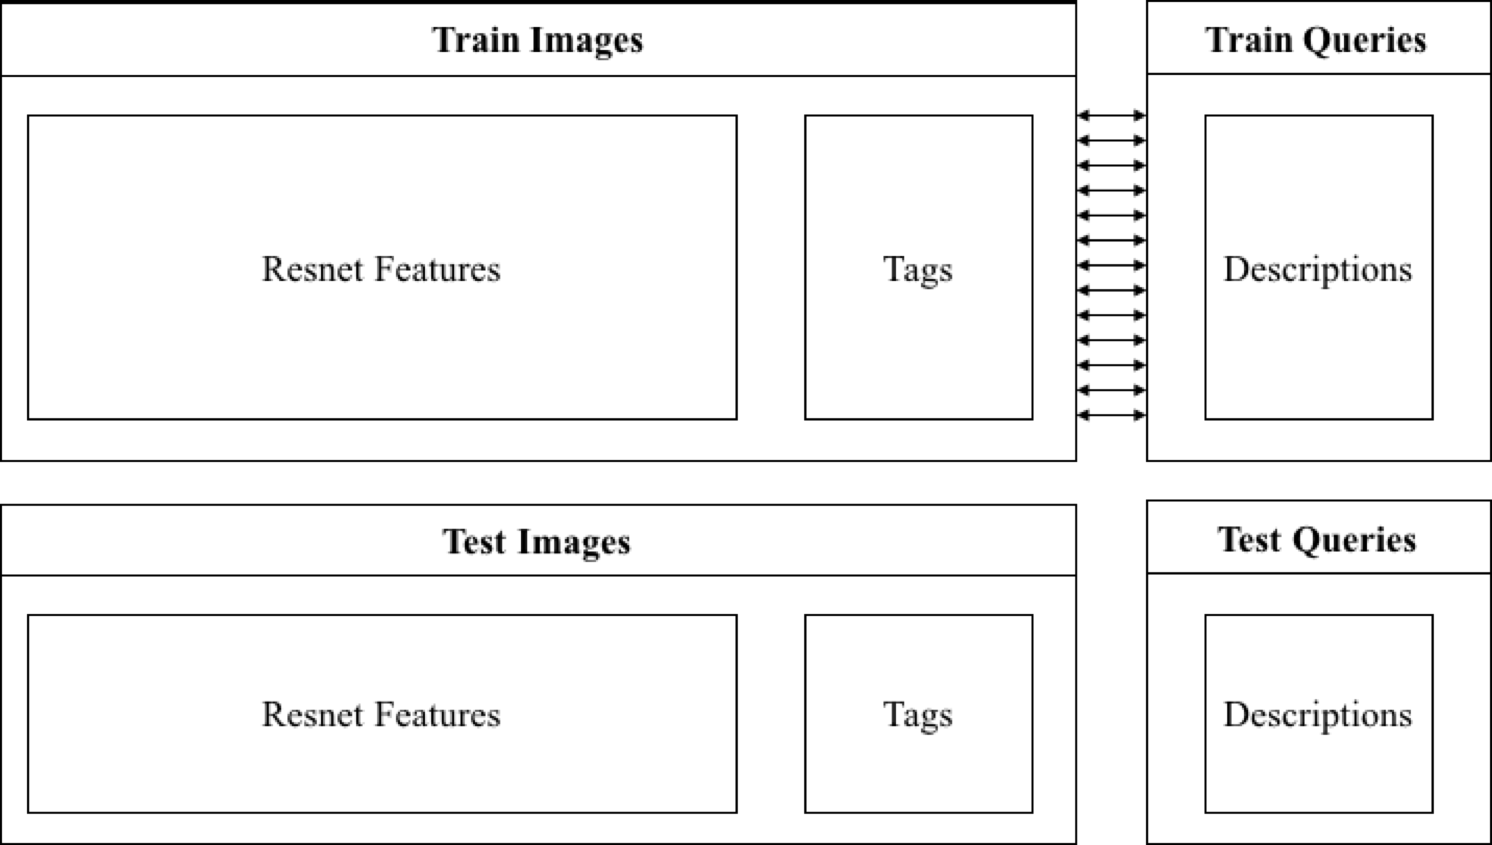
\includegraphics[width=0.9\textwidth]{schematic.png}
   \caption{Schematic Representation of Data Provided}
   \centering
\end{figure}

\subsubsection*{Queries to Image Approach}
\addcontentsline{toc}{subsubsection}{Queries to Image Approach}

By mapping test queries to train queries, we get the corresponding train images since there is a one-to-one relationship in the training data. For these images, if we find the most similar test images using image ResNet features and image tags provided. This allowed us to create a mapping between test queries and test images. We found that this general approach yielded better results than the Queries to Image Approach. \\ 

Test description  $\rightarrow$   Closest Matching Train Description  $\rightarrow$  Train Image  $\rightarrow$  20 Most Similar Test Images

\subsubsection*{Image to Queries Approach}
\addcontentsline{toc}{subsubsection}{Image to Queries Approach}

For each testing image, if we find a set of similar training images, we can access their descriptions to create an aggregate description for a given testing image. We can then calculate pairwise similarities between aggregate descriptions for the test images and test descriptions. Using these similarity scores, we can arrive at a set of top matches for each test description. This approach leaded to lower results. \\


Test Image $\rightarrow$  Similar Train Images $\rightarrow$ Train Description $\rightarrow$ Aggregate Description <similarity scores> Test Descriptions 


\subsection*{Description-to-Image KNN Model}
\addcontentsline{toc}{subsection}{Description-to-Image KNN Model}

\subsubsection*{Data Representation}
\addcontentsline{toc}{subsubsection}{Data Representation}

We parsed the training and testing feature set for the final Resnet layer fc1000. We processed descriptions by removing all punctuations, lowercasing all words, removing stopwords and lemmatizing all words using NLTK's Porter Stemmer. We then created a dictionary of all words appearing more than 10 times in training and testing descriptions. We built a bag of words representation of training and testing descriptions using the dictionary. We also performed L2 normalization on the training and testing description features to normalize the vectors.


\subsubsection*{Algorithm}
\addcontentsline{toc}{subsubsection}{Algorithm}

We used scikit-learn's kNN classifier to fit training description features to image names. For each test description feature, used the .predict method in scikit-learn on the KNN classifier (n\_neighbor=1)  to get the closest training description based on the description feature vector. Since this directly mapped to a training image, we could get the corresponding ResNet training feature vector for that image. We then computed similarity scores for the testing image ResNet fc1000 feature vectors using a distance function to the training image ResNet fc1000 feature vector. We experimented with cosine similarity and euclidean distance as similarity measures. We found that using cosine similarity provided better scores than using the euclidean distance. For each test feature/label combination, we find by the lowest 20 scores (closest test features) and return the test image labels associated with them to be used for submission.


\subsection*{Image-to-Description Model}
\addcontentsline{toc}{subsection}{Image-to-Description Model}

\subsubsection*{Data Representation}
\addcontentsline{toc}{subsubsection}{Data Representation}
Similar to the approach for the Description-to-Image model, we preprocessed the descriptions and built a bag of words model for the training and testing descriptions.

\subsubsection*{Algorithm}
\addcontentsline{toc}{subsubsection}{Algorithm}

For each testing image, we find two closest training images by computing the cosine similarities between our test image and the training images using the 100 ResNet fc1000 features. We then compute the aggregated description feature vector based on the nearest training images. We built a map of the testing image to its aggregated description feature. For each test description feature, we then find the top 20 aggregated description feature associated with the testing images using the euclidean (L2) distance between the aggregated description feature and the testing feature vectors. When finding the distance between the description feature vectors in training and testing data, using the euclidean distance provided better measures than using the cosine similarity function.


\subsection*{Similarity Mapping}
\addcontentsline{toc}{subsection}{Similarity Mapping}


\subsubsection*{Data Representation}
\addcontentsline{toc}{subsubsection}{Data Representation}
We used the same data representation as in the Description-to-Image model for this approach. In addition, we also cleaned and projected the tags data on images to a 80-dimensional bag of words vectors.

\subsubsection*{Algorithm}
\addcontentsline{toc}{subsubsection}{Algorithm}
We calculated similarities between testing description vectors and training description vectors using cosine similarities. For each testing description vector we found $n_1$ training description vectors that closely matched. For each of these $n_1$ corresponding training images, we used ResNet fc1000 + 80-dimensional tags data as features to calculate cosine similarity with testing images. We then found $n_2$ testing images for each of these $n_1$ training images with highest similarity scores, while maintaining $n_1$ x $n_2$ = 20. We found that $n_1$=4 and $n_2$=5 works best for our Kaggle submission scores. In addition to cosine similarity, we tried euclidean and euclidean-weighted-cosine similarities. We found that cosine similarities yielded the best results for matching both description vectors and image vectors. \\

In addition to the ($n_1$,$n_2$) approach used above, we also tried to use similarity chaining, by creating a combined similarity score as net\_similarity = description\_similiarity x image\_similiarity. We found that this approach did not improve on the results of the ($n_1$,$n_2$) approach. \\

Test descriptions <similarity scores>  Train Descriptions $\rightarrow$ Train Images  <similarity scores> Test Images


\subsection*{Predicting Descriptions}
\addcontentsline{toc}{subsection}{Predicting Descriptions}

If we could create a statistical model that mapped training image features to training descriptions, we could predict descriptions given a training image. We could use these to calculate similarities like in the Image-to-Query approach above. Note that unlike the approach above, this does not look at similarities between test and train images explicitly.

\subsubsection*{Data Representation}
\addcontentsline{toc}{subsubsection}{Data Representation}
We cleaned the descriptions data as above through lemmatizing, removing stopwords etc. For projecting descriptions as vectors, we used gensim's Doc2Vec module to create document embeddings out of this cleaned text with 100 dimensions and 100 training epochs.

\subsubsection*{Algorithm}
\addcontentsline{toc}{subsubsection}{Algorithm}
We used ResNet fc1000 and bag of words as input features for our model. We built a sequential neural network and trained it with training images and training description data. Given a test image vector, the goal was to predict description vector as output. We tried various configurations of the network through change in number of layers, neurons per layer, activation functions, use of drop out to prevent overfitting, various optimizers and learning rates to tune the model. Here are the specifications of the final model: 

\begin{itemize}
	\item Module: Keras on TensorFlow backend 
	\item Input Layer: 1080 neurons, linear activation
	\item Second Layer: 1620 neurons, linear activation, dropout=0.1
	\item Third Layer: 500 neurons, reLU activation
	\item Output Layer: 100 neurons, linear activation
\end{itemize} 

Learning rate=0.01, Optimizer= adam, Loss function: mean squared error, Epochs=50 \\

We found that the results of the description predictions were dismal on manual review. Increasing the neural network architecture added to the computational workload, and made running it on local machines not feasible. We looked into using Google Cloud platform for training larger networks, but decided not to in the interest of limited time.



\section*{Results \& Conclusion}
\addcontentsline{toc}{section}{Results  \& Conclusion}


\begin{center}
\begin{tabular}{ | L | L | L |  }
\hline
 Approach & Public Leaderboard
Kaggle Score & Private Leaderboard
Kaggle Score \\ 
 \hline
Description-to-Image KNN Model & 0.13235 & 0.13631 \\
 \hline
 Similarity Mapping & 0.13442 & 0.1406  \\
 \hline
 Image-to-Description Model & 0.17067 & 0.14690  \\
 \hline
 Similarity Mapping & 0.22709 & 0.21257  \\
 \hline
\end{tabular}
\end{center}


We found that the Image-to-description approach yielded the best results. Using euclidean distance to find the closest descriptions based on bag-of-words allowed us to generate a more accurate representation of the target image for a given description. \\ 

After trying various representations of the data, we found that using the ResNet fc1000 features along with tags as bag of words features out performs ResNet fc1000 or tags alone in isolation in image-to-image matching.  \\

We believe that we could improve image to image matching by using intermediate pool ResNet layers. We are still inclined towards exploring document embeddings to improve our description matching. In addition, using methods like neural networks or SVMs to model relationships between image features and text features seems like a plausible future direction. \\


\newpage

\section*{Background  \& Related Work}
\addcontentsline{toc}{section}{Background  \& Related Work}

Wang, Baiyang, and Diego Klabjan. ?An Attention-Based Deep Net for Learning to Rank.? [1702.06106] \textit{An Attention-Based Deep Net for Learning to Rank}, 15 May 2017, \url{arxiv.org/abs/1702.06106}.
\newline
\newline


Li, Yuncheng, et al. ?Improving Pairwise Ranking for Multi-Label Image Classification.? [1704.03135] \textit{Improving Pairwise Ranking for Multi-Label Image Classification}, 1 June 2017, \url{arxiv.org/abs/1704.03135}.
\newline
\newline


Mitra, Bhaskar, and Nick Craswell. ?Neural Models for Information Retrieval.? [1705.01509] \textit{Neural Models for Information Retrieval}, 3 May 2017, \url{arxiv.org/abs/1705.01509}.
\newline
\newline

Wang, Liwei, et al. ?Learning Deep Structure-Preserving Image-Text Embeddings.? [1511.06078] \textit{Learning Deep Structure-Preserving Image-Text Embeddings}, 14 Apr. 2016, \url{arxiv.org/abs/1511.06078}.
\newline
\newline


Palangi, Hamid, et al. ?Deep Sentence Embedding Using Long Short-Term Memory Networks: Analysis and Application to Information Retrieval.? [1502.06922] \textit{Deep Sentence Embedding Using Long Short-Term Memory Networks: Analysis and Application to Information Retrieval}, 16 Jan. 2016, \url{arxiv.org/abs/1502.06922}.
\newline
\newline


Le, Quoc V., and Tomas Mikolov. ?Distributed Representations of Sentences and Documents.? [1405.4053] \textit{Distributed Representations of Sentences and Documents}, 22 May 2014, \url{arxiv.org/abs/1405.4053}.
\newline
\newline



\newpage




%-------------------------------------------------------------------------------
% REFERENCES
%-------------------------------------------------------------------------------
\newpage
\section*{Sources \& External libraries}
\addcontentsline{toc}{section}{Sources \& External libraries}

St�fan van der Walt, S. Chris Colbert and Ga�l Varoquaux. \textit{The NumPy Array: A Structure for Efficient Numerical Computation}, Computing in Science \& Engineering, 13, 22-30 (2011), DOI:10.1109/MCSE.2011.37
\newline
\newline

John D. Hunter. \textit{Matplotlib: A 2D Graphics Environment}, Computing in Science \& Engineering, 9, 90-95 (2007), DOI:10.1109/MCSE.2007.55
\newline
\newline


Wes McKinney. \textit{Data Structures for Statistical Computing in Python}, Proceedings of the 9th Python in Science Conference, 51-56 (2010)
\newline
\newline

Fabian Pedregosa, Ga�l Varoquaux, Alexandre Gramfort, Vincent Michel, Bertrand Thirion, Olivier Grisel, Mathieu Blondel, Peter Prettenhofer, Ron Weiss, Vincent Dubourg, Jake Vanderplas, Alexandre Passos, David Cournapeau, Matthieu Brucher, Matthieu Perrot, �douard Duchesnay. \textit{Scikit-learn: Machine Learning in Python}, Journal of Machine Learning Research, 12, 2825-2830 (2011)
\newline
\newline

Jones E, Oliphant E, Peterson P, et al. \textit{SciPy: Open Source Scientific Tools for Python}, 2001-, \url{http://www.scipy.org/}
\newline
\newline

"A Gentle Introduction to the Bag-Of-Words Model."  \textit{Machine Learning Mastery}, 20 Nov. 2017, \url{machinelearningmastery.com/gentle-introduction-bag-words-model/}.
\newline
\newline

\textit{What is the difference between bag of words, TF-IDF, and vector space model?}, \url{www.quora.com/What-is-the-difference-between-bag-of-words-TF-IDF-and-vector-space-model}.
\newline
\newline

C., Gab. "Bag of Words and Tf-Idf Explained." \textit{Data Meets Media}, 7 May 2017, \url{datameetsmedia.com/bag-of-words-tf-idf-explained/}.
\newline
\newline


\end{document}

%-------------------------------------------------------------------------------
% SNIPPETS
%-------------------------------------------------------------------------------

%\begin{figure}[!ht]
%   \centering
%   \includegraphics[width=0.8\textwidth]{file_name}
%   \caption{}
%   \centering
%   \label{label:file_name}
%\end{figure}

%\begin{figure}[!ht]
%   \centering
%   \includegraphics[width=0.8\textwidth]{graph}
%   \caption{Blood pressure ranges and associated level of hypertension (American Heart Association, 2013).}
%   \centering
%   \label{label:graph}
%\end{figure}

%\begin{wrapfigure}{r}{0.30\textwidth}
%   \vspace{-40pt}
%   \begin{center}
%       \includegraphics[width=0.29\textwidth]{file_name}
%   \end{center}
%   \vspace{-20pt}
%   \caption{}
%   \label{label:file_name}
%\end{wrapfigure}

%\begin{wrapfigure}{r}{0.45\textwidth}
%   \begin{center}
%       \includegraphics[width=0.29\textwidth]{manometer}
%   \end{center}
%   \caption{Aneroid sphygmomanometer with stethoscope (Medicalexpo, 2012).}
%   \label{label:manometer}
%\end{wrapfigure}

%\begin{table}[!ht]\footnotesize
%   \centering
%   \begin{tabular}{cccccc}
%   \toprule
%   \multicolumn{2}{c} {Pearson's correlation test} & \multicolumn{4}{c} {Independent t-test} \\
%   \midrule    
%   \multicolumn{2}{c} {Gender} & \multicolumn{2}{c} {Activity level} & \multicolumn{2}{c} {Gender} \\
%   \midrule
%   Males & Females & 1st level & 6th level & Males & Females \\
%   \midrule
%   \multicolumn{2}{c} {BMI vs. SP} & \multicolumn{2}{c} {Systolic pressure} & \multicolumn{2}{c} {Systolic Pressure} \\
%   \multicolumn{2}{c} {BMI vs. DP} & \multicolumn{2}{c} {Diastolic pressure} & \multicolumn{2}{c} {Diastolic pressure} \\
%   \multicolumn{2}{c} {BMI vs. MAP} & \multicolumn{2}{c} {MAP} & \multicolumn{2}{c} {MAP} \\
%   \multicolumn{2}{c} {W:H ratio vs. SP} & \multicolumn{2}{c} {BMI} & \multicolumn{2}{c} {BMI} \\
%   \multicolumn{2}{c} {W:H ratio vs. DP} & \multicolumn{2}{c} {W:H ratio} & \multicolumn{2}{c} {W:H ratio} \\
%   \multicolumn{2}{c} {W:H ratio vs. MAP} & \multicolumn{2}{c} {\% Body fat} & \multicolumn{2}{c} {\% Body fat} \\
%   \multicolumn{2}{c} {} & \multicolumn{2}{c} {Height} & \multicolumn{2}{c} {Height} \\
%   \multicolumn{2}{c} {} & \multicolumn{2}{c} {Weight} & \multicolumn{2}{c} {Weight} \\
%   \multicolumn{2}{c} {} & \multicolumn{2}{c} {Heart rate} & \multicolumn{2}{c} {Heart rate} \\
%   \bottomrule
%   \end{tabular}
%   \caption{Parameters that were analysed and related statistical test performed for current study. BMI - body mass index; SP - systolic pressure; DP - diastolic pressure; MAP - mean arterial pressure; W:H ratio - waist to hip ratio.}
%   \label{label:tests}
%\end{table}